\documentclass[12pt]{article}

\title{Natural caustics in backward path tracing}
\author{
Shawn Halayka\footnote{sjhalayka@gmail.com}
}


\date{\today\;\currenttime}

\usepackage{datetime}
\usepackage{listings}
\usepackage{cite}
\usepackage{xcolor}
\usepackage{graphicx}
\usepackage{setspace}
\usepackage{amsmath}
\usepackage{url}
\usepackage{amsfonts}
\usepackage{caption}
\usepackage{subcaption}

\usepackage[margin=1in]{geometry}

%\doublespace

\begin{document}

\newcommand{\abs}[1]{\lvert#1\rvert}



\maketitle




\begin{abstract}
In this paper we introduce a natural method for producing both refraction and reflection caustics in backward path tracing (e.g. bouncing around an eye ray in the scene until a light is found).
These caustics do not rely on a light location, and as such, do not rely on bidirectional or forward path tracing.
As such, these caustics allow for as many light sources as one would care for; the shapes and positions of the lights are completely arbitrary (can be bunny shaped, etc).
We use the standard Cornell box for testing the backward path tracer.
\end{abstract}

\section{Rasterizer versus ray tracing versus backward path tracing}

Here we rate the three main visualization algorithms.
We rate them in terms of what is relatively easy, or naturally occurring, in each of the visualization algorithms.
\begin{center}
\begin{tabular}{| l | r | r | r | r |}
  \hline
 Algorithm &  Reflections & Shadows & Refraction caustics & Reflection caustics \\
\hline
\hline
Rasterizer & No & No & No &  No \\
Ray tracer & Yes & Sharp & No & No  \\
Backward path tracer & Yes & Sharp / soft & Yes & Yes \\
  \hline  
\end{tabular}
\end{center}
Clearly, the most suitable visualization algorithm for now (and in the future) is the backward path tracer.
This not to say that, for instance in the case of the rasterizer, there is no such thing as shadows.
It's just that the implementation of shadows is a kludgy affair, or not naturally occurring.

Although caustics can be produced using forward or bidirectional path tracing, they suffer from convergence (or lack thereof) problems.
These issues do not plague the backward path tracer.





\section{Path tracer code}
A full Vulkan code exists \cite{halayka}, using a very simple (e.g. not physically accurate) light transport algorithm.
The results given here can only get better with the improvement of the light transport algorithm.
This code is based off of Sascha Willems' work \cite{willems1, willems2}.



\section{Acknowledgement}

The Cornell boxes used in this paper were developed by Rob Rau.






\begin{thebibliography}{9}

\bibitem{kajiya} Kajiya. The rendering equation.
\bibitem{halayka} Halayka. Vulkan code. \url{https://github.com/sjhalayka/cornell_box_textured}
\bibitem{willems1} Willems. Path tracer code. \url{https://github.com/SaschaWillems/VulkanPathTracer}
\bibitem{willems2} Willems. Vulkan demo codes. \url{https://github.com/SaschaWillems/Vulkan}


\end{thebibliography}


\pagebreak




\begin{figure} 
\centering
  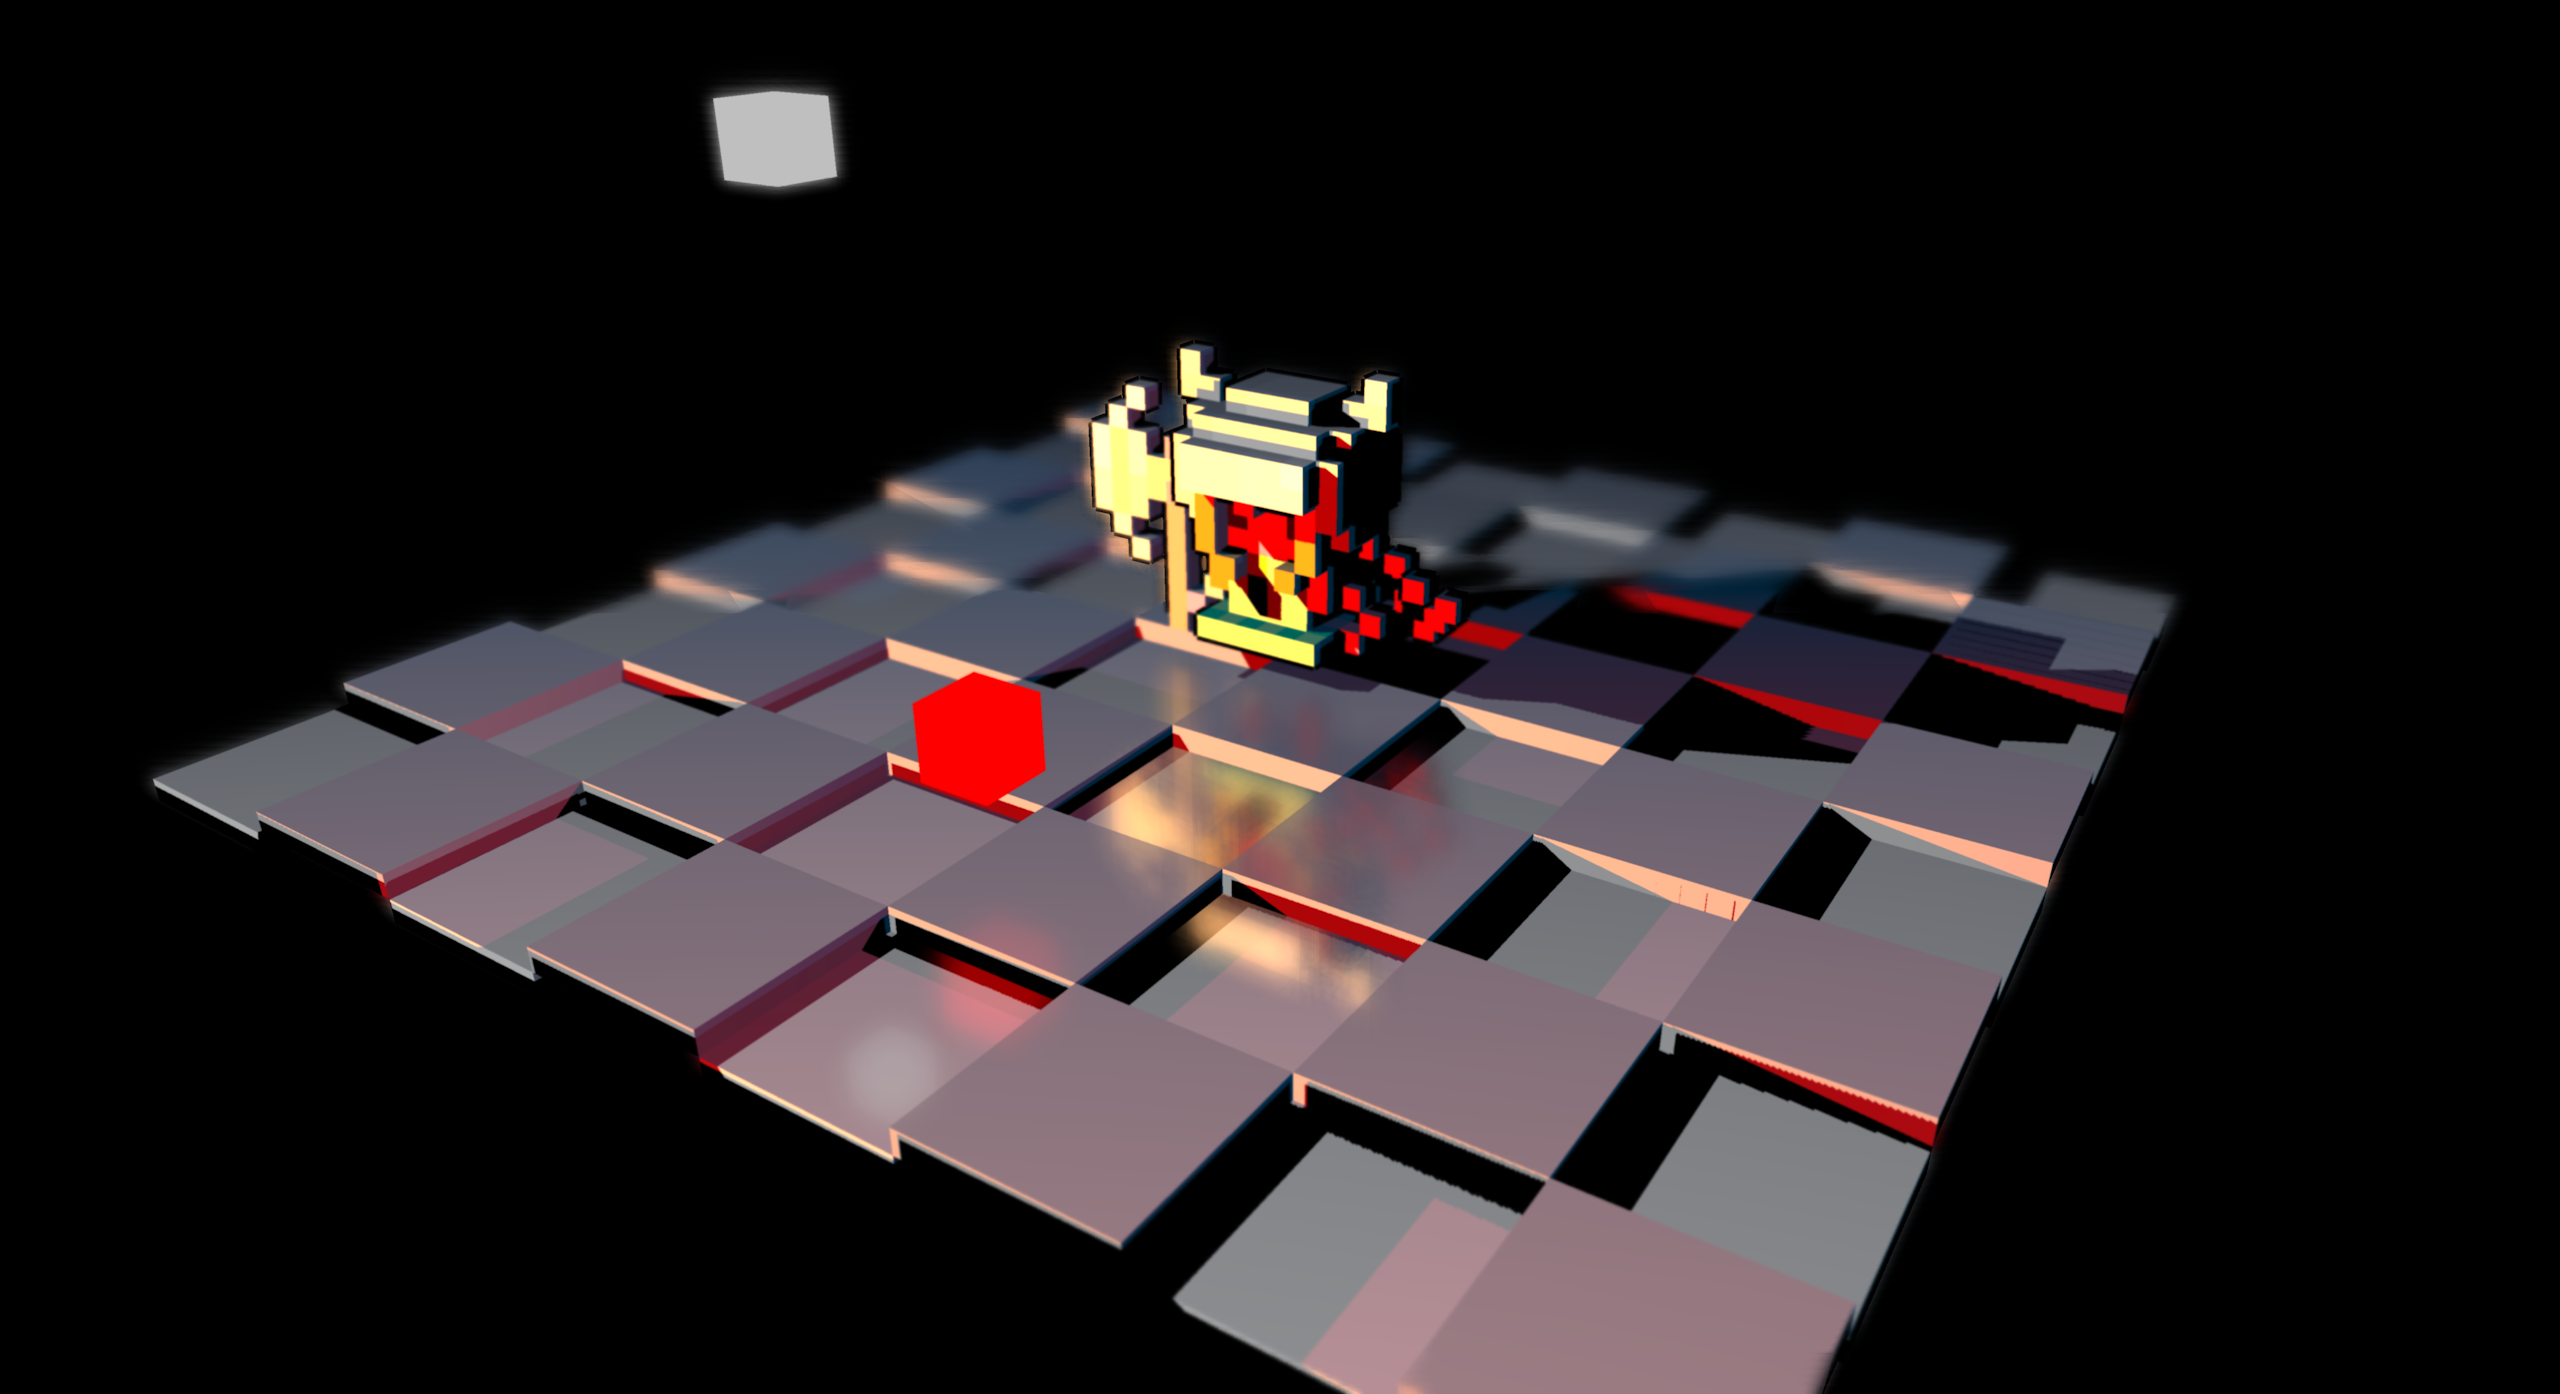
\includegraphics[width = 6 in]{rasterizer.png}
  \caption{ Rasterizer.
The surface is lit using Phong shading and omnidirectional shadow maps.
The reflections are faked -- the camera is flipped upside down, and reflected things masked and drawn.
In other words, reflections and shadows are not naturally occurring.
Global illumination is not taken into account.
This knight model, as well as MagicaVoxel, were made by the Twitter user @ephtracy.
}

\end{figure}




\begin{figure} 
\centering
  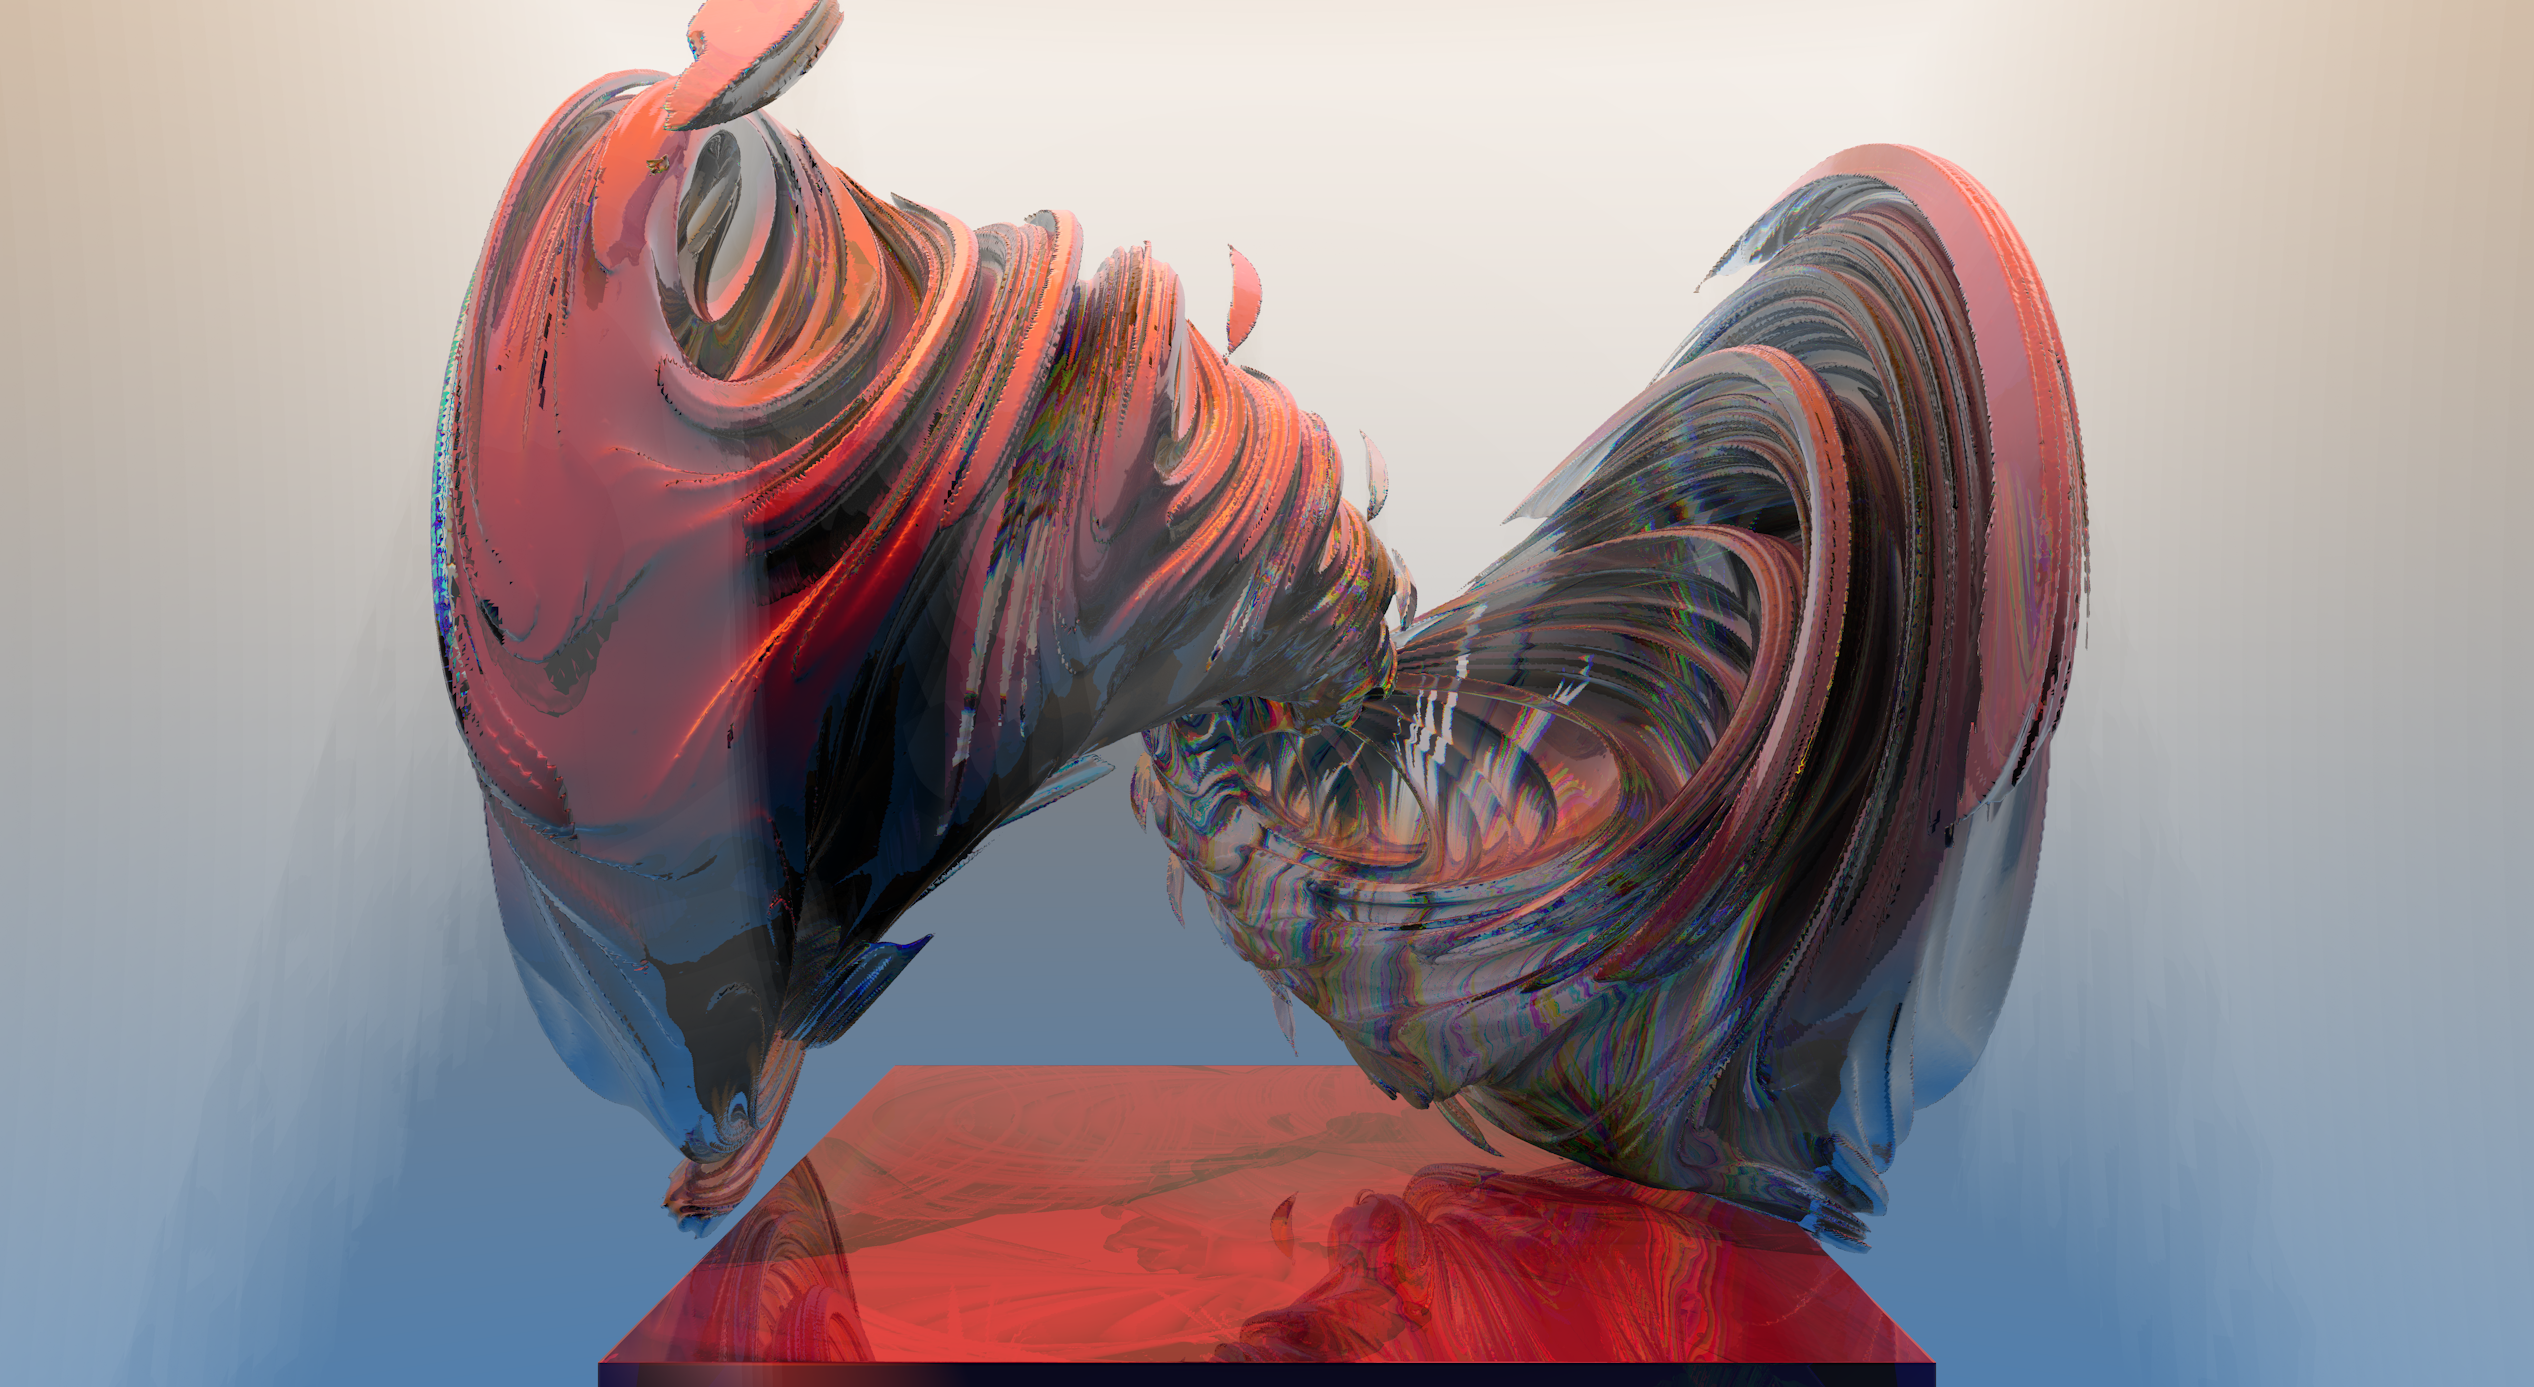
\includegraphics[width = 6 in]{v_rt_reflect.png}
  \caption{ Ray tracer, taking into account transparency.
The surface is lit using Phong shading and sharp shadows.
In other words, reflections and shadows are naturally occurring.
Global illumination is not taken into account.
}
\end{figure}


\begin{figure} 
\centering
  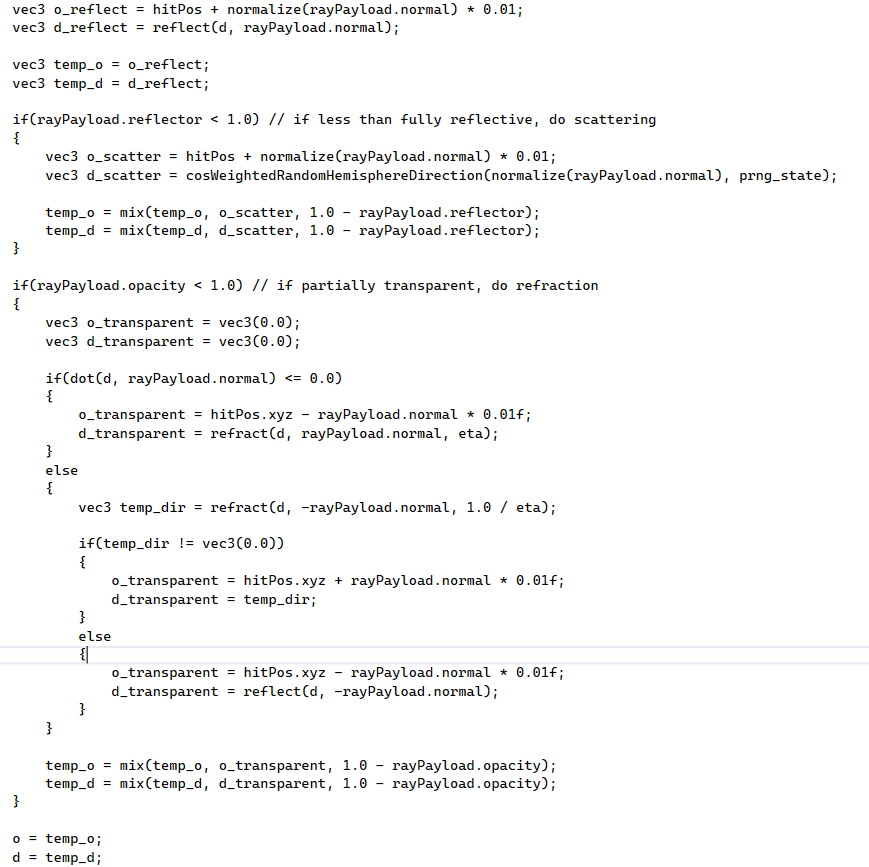
\includegraphics[width = 6 in]{code.png}
  \caption{ Taking transparent objects into consideration.
In essence, instead of always producing a pseudorandom cosine-weighted reflection vector, refraction occurs for transparent objects.
}
\end{figure}

\begin{figure} 
\centering
  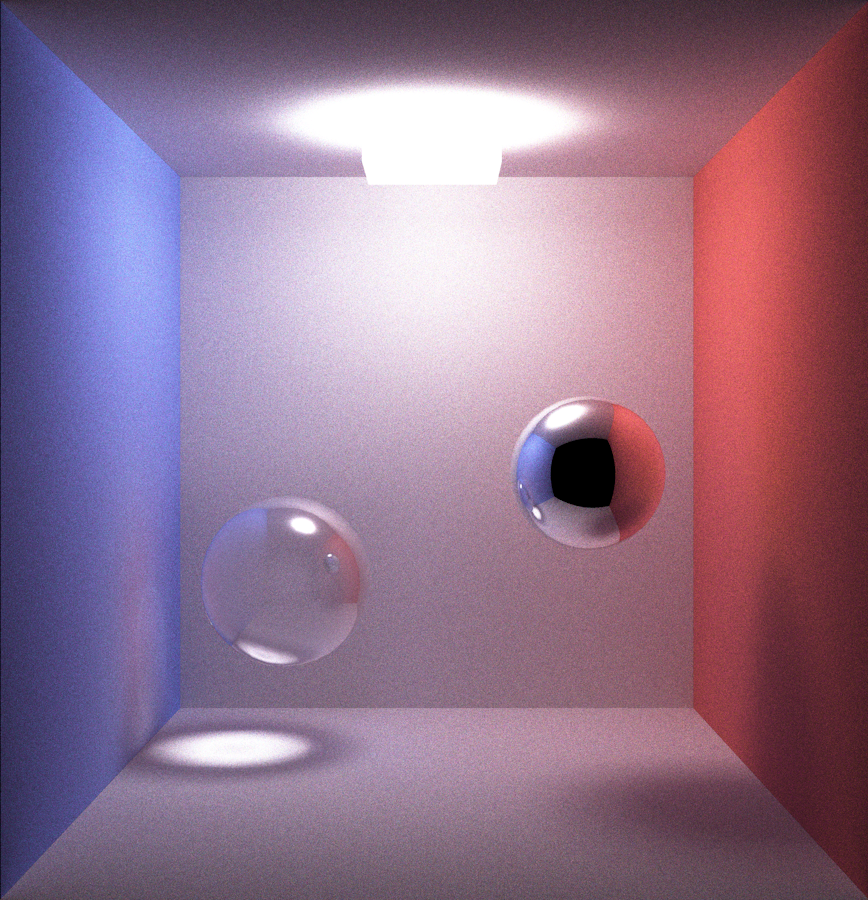
\includegraphics[width = 6 in]{v_rt_reflect_no_chromatic_aberration_low_res.png}
  \caption{  Backward path tracer, taking transparent objects into consideration. 
Note the naturally occurring refraction caustic.
Note the soft shadows.
Global illumination (e.g. colour bleeding / indirect lighting) is taken into account.
}
\end{figure}


\begin{figure} 
\centering
  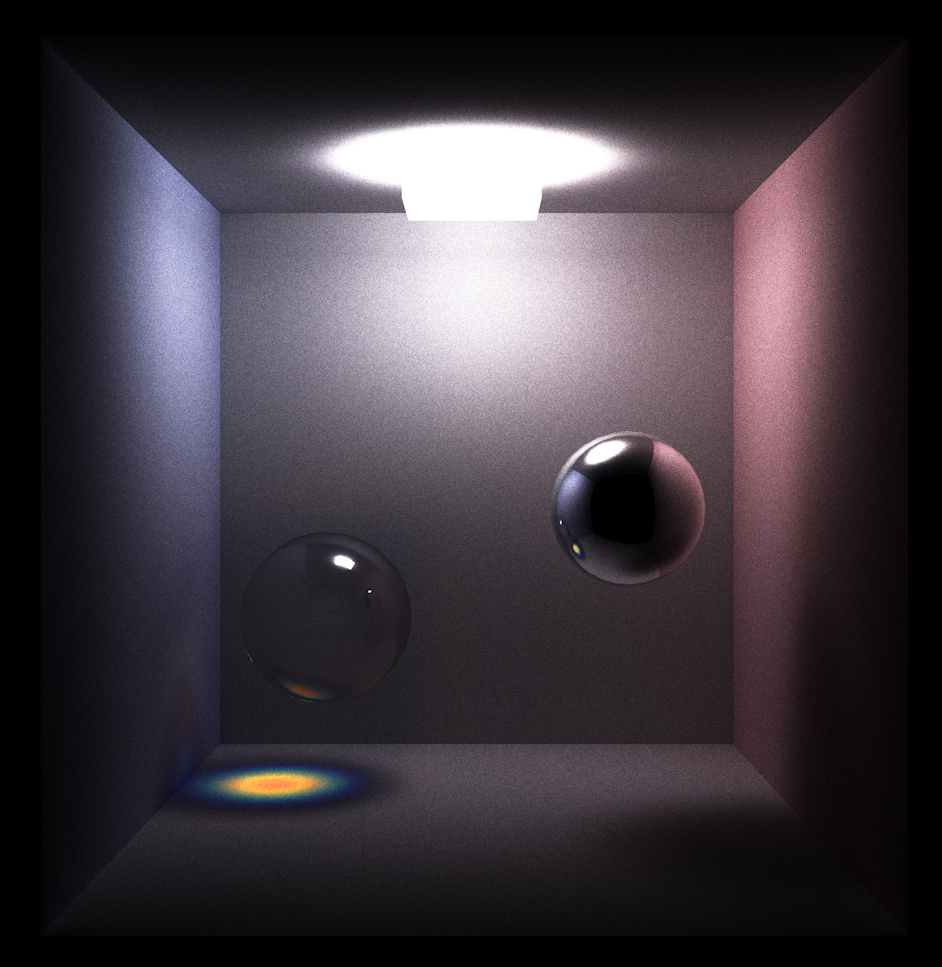
\includegraphics[width = 6 in]{v_rt_reflect_chromatic_aberration_low_res.png}
  \caption{ Note the refraction caustic, with 3-channel chromatic aberration.
}
\end{figure}

\begin{figure} 
\centering
  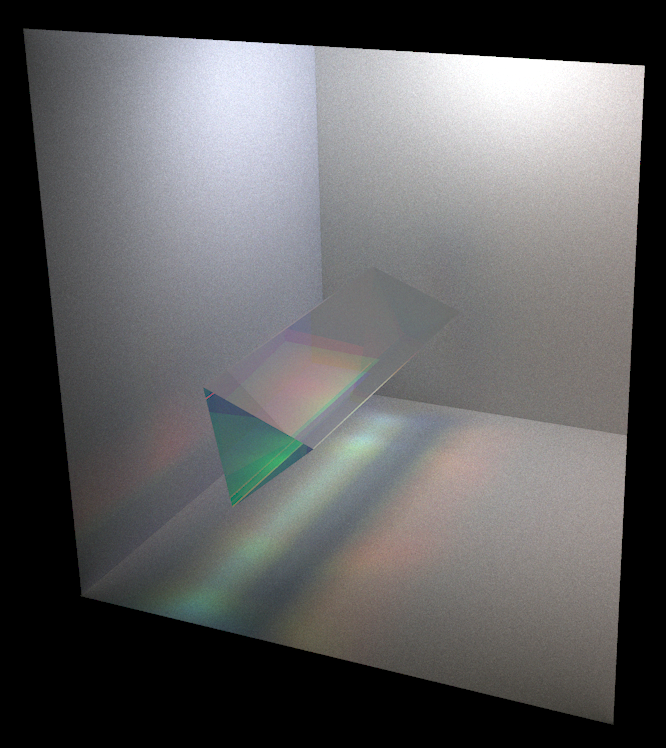
\includegraphics[width = 6 in]{v_rt_reflect_prism.png}
  \caption{ Note the refraction caustic, with 3-channel chromatic aberration.
}
\end{figure}


\begin{figure} 
\centering
  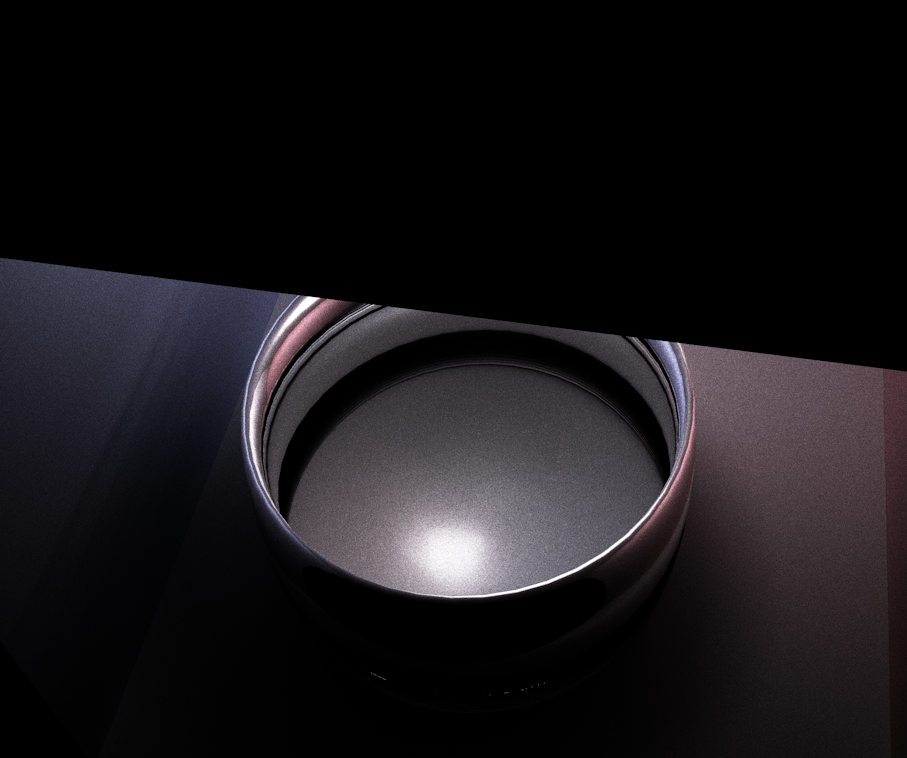
\includegraphics[width = 6 in]{v_rt_reflection_caustic.png}
  \caption{ Note the reflection caustic.
}
\end{figure}






\end{document}









